\noindent
La simulación computacional se ha consolidado como una herramienta fundamental
en el desarrollo y validación de sistemas de conducción autónoma.
Permite recrear escenarios complejos y potencialmente peligrosos de manera segura,
flexible y económica, facilitando la experimentación y el análisis de algoritmos
antes de su implementación en vehículos reales. En el contexto de este trabajo,
la simulación resulta especialmente útil para modelar situaciones de estacionamiento
automático, donde la precisión y la seguridad son críticas. A través de la simulación,
es posible ajustar parámetros, evaluar el desempeño de sensores virtuales y analizar el
comportamiento del sistema bajo diferentes condiciones ambientales y de tráfico,
todo ello sin los riesgos y costos asociados a las pruebas físicas.
La simulación puede proporcionar información detallada sobre el vehículo y
su entorno, lo que permite realizar mediciones y análisis exhaustivos de los
datos obtenidos, de manera similar a como se haría en la vida real.
\noindent
En este trabajo se emplean plataformas y bibliotecas ampliamente adoptadas en visión
por computadora y simulación para vehículos autónomos.
En particular, utilizamos CARLA, un simulador de código abierto que permite recrear entornos urbanos realistas
con agentes dinámicos y sensores virtuales configurables, y OpenCV, una biblioteca de procesamiento
de imágenes que proporciona las operaciones básicas para umbralización, detección de bordes (Canny)
y detección de líneas (Hough), entre otras.

\subsubsection{CARLA Simulator}\label{sec:carla-teorico}
\noindent
CARLA (Car Learning to Act) es una plataforma orientada a investigación que facilita la generación de escenas
complejas y controladas, con variabilidad de clima, iluminación y tráfico, y un conjunto de sensores virtuales
(cámaras, LiDAR, radar, GPS) que producen datos cercanos a los de un vehículo real.
Su flexibilidad para instrumentar escenarios y capturar datos reproducibles lo hace idóneo para
experimentación y validación de algoritmos de percepción, localización y control en contextos como el
estacionamiento automático \cite{dosovitskiy2017carla}.
En la Sección \ref{subsec:simulation-design} se detalla el diseño específico del entorno de simulación que
utilizamos, y en la Figura~\ref{fig:carla-simulator-teo} (véase Sección \ref{sec:carla-teorico}) se ilustran ejemplos
de condiciones ambientales configurables en la plataforma.

\begin{figure}[!ht]
	\centering
	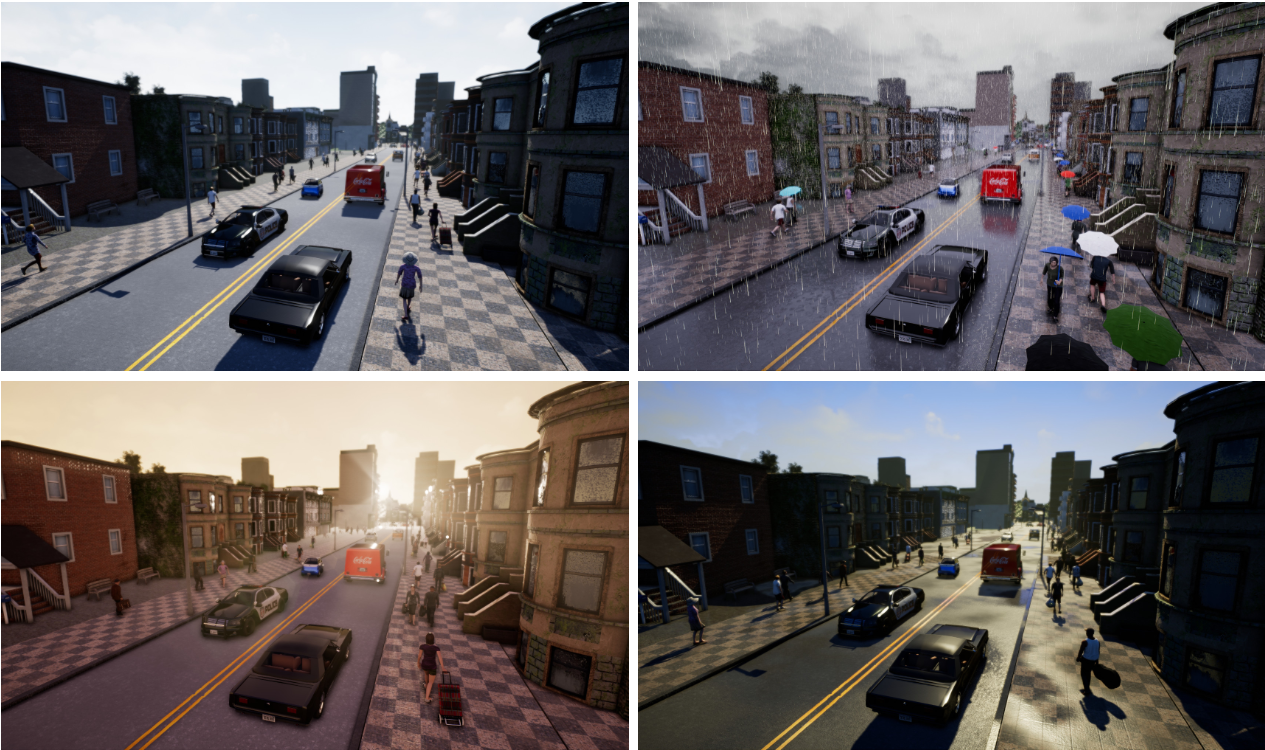
\includegraphics[width=0.8\textwidth]{img/carla_clima_example}
	\caption{Ejemplos de condiciones ambientales configurables en el simulador CARLA.}
	\label{fig:carla-simulator-teo}
\end{figure}

\subsubsection{OpenCV}
\noindent
OpenCV proporciona el conjunto de operaciones y estructuras necesarias para el preprocesado de imágenes y la extracción de primitivas geométricas, incluyendo umbralización, Canny y la transformada de Hough, que se emplean en la detección de la retícula de estacionamiento.
